% Options for packages loaded elsewhere
\PassOptionsToPackage{unicode}{hyperref}
\PassOptionsToPackage{hyphens}{url}
%
\documentclass[
]{book}
\usepackage{lmodern}
\usepackage{amssymb,amsmath}
\usepackage{ifxetex,ifluatex}
\ifnum 0\ifxetex 1\fi\ifluatex 1\fi=0 % if pdftex
  \usepackage[T1]{fontenc}
  \usepackage[utf8]{inputenc}
  \usepackage{textcomp} % provide euro and other symbols
\else % if luatex or xetex
  \usepackage{unicode-math}
  \defaultfontfeatures{Scale=MatchLowercase}
  \defaultfontfeatures[\rmfamily]{Ligatures=TeX,Scale=1}
\fi
% Use upquote if available, for straight quotes in verbatim environments
\IfFileExists{upquote.sty}{\usepackage{upquote}}{}
\IfFileExists{microtype.sty}{% use microtype if available
  \usepackage[]{microtype}
  \UseMicrotypeSet[protrusion]{basicmath} % disable protrusion for tt fonts
}{}
\makeatletter
\@ifundefined{KOMAClassName}{% if non-KOMA class
  \IfFileExists{parskip.sty}{%
    \usepackage{parskip}
  }{% else
    \setlength{\parindent}{0pt}
    \setlength{\parskip}{6pt plus 2pt minus 1pt}}
}{% if KOMA class
  \KOMAoptions{parskip=half}}
\makeatother
\usepackage{xcolor}
\IfFileExists{xurl.sty}{\usepackage{xurl}}{} % add URL line breaks if available
\IfFileExists{bookmark.sty}{\usepackage{bookmark}}{\usepackage{hyperref}}
\hypersetup{
  pdftitle={Comparative Methods Workshops},
  pdfauthor={Chris Mitchell},
  hidelinks,
  pdfcreator={LaTeX via pandoc}}
\urlstyle{same} % disable monospaced font for URLs
\usepackage{color}
\usepackage{fancyvrb}
\newcommand{\VerbBar}{|}
\newcommand{\VERB}{\Verb[commandchars=\\\{\}]}
\DefineVerbatimEnvironment{Highlighting}{Verbatim}{commandchars=\\\{\}}
% Add ',fontsize=\small' for more characters per line
\usepackage{framed}
\definecolor{shadecolor}{RGB}{248,248,248}
\newenvironment{Shaded}{\begin{snugshade}}{\end{snugshade}}
\newcommand{\AlertTok}[1]{\textcolor[rgb]{0.94,0.16,0.16}{#1}}
\newcommand{\AnnotationTok}[1]{\textcolor[rgb]{0.56,0.35,0.01}{\textbf{\textit{#1}}}}
\newcommand{\AttributeTok}[1]{\textcolor[rgb]{0.77,0.63,0.00}{#1}}
\newcommand{\BaseNTok}[1]{\textcolor[rgb]{0.00,0.00,0.81}{#1}}
\newcommand{\BuiltInTok}[1]{#1}
\newcommand{\CharTok}[1]{\textcolor[rgb]{0.31,0.60,0.02}{#1}}
\newcommand{\CommentTok}[1]{\textcolor[rgb]{0.56,0.35,0.01}{\textit{#1}}}
\newcommand{\CommentVarTok}[1]{\textcolor[rgb]{0.56,0.35,0.01}{\textbf{\textit{#1}}}}
\newcommand{\ConstantTok}[1]{\textcolor[rgb]{0.00,0.00,0.00}{#1}}
\newcommand{\ControlFlowTok}[1]{\textcolor[rgb]{0.13,0.29,0.53}{\textbf{#1}}}
\newcommand{\DataTypeTok}[1]{\textcolor[rgb]{0.13,0.29,0.53}{#1}}
\newcommand{\DecValTok}[1]{\textcolor[rgb]{0.00,0.00,0.81}{#1}}
\newcommand{\DocumentationTok}[1]{\textcolor[rgb]{0.56,0.35,0.01}{\textbf{\textit{#1}}}}
\newcommand{\ErrorTok}[1]{\textcolor[rgb]{0.64,0.00,0.00}{\textbf{#1}}}
\newcommand{\ExtensionTok}[1]{#1}
\newcommand{\FloatTok}[1]{\textcolor[rgb]{0.00,0.00,0.81}{#1}}
\newcommand{\FunctionTok}[1]{\textcolor[rgb]{0.00,0.00,0.00}{#1}}
\newcommand{\ImportTok}[1]{#1}
\newcommand{\InformationTok}[1]{\textcolor[rgb]{0.56,0.35,0.01}{\textbf{\textit{#1}}}}
\newcommand{\KeywordTok}[1]{\textcolor[rgb]{0.13,0.29,0.53}{\textbf{#1}}}
\newcommand{\NormalTok}[1]{#1}
\newcommand{\OperatorTok}[1]{\textcolor[rgb]{0.81,0.36,0.00}{\textbf{#1}}}
\newcommand{\OtherTok}[1]{\textcolor[rgb]{0.56,0.35,0.01}{#1}}
\newcommand{\PreprocessorTok}[1]{\textcolor[rgb]{0.56,0.35,0.01}{\textit{#1}}}
\newcommand{\RegionMarkerTok}[1]{#1}
\newcommand{\SpecialCharTok}[1]{\textcolor[rgb]{0.00,0.00,0.00}{#1}}
\newcommand{\SpecialStringTok}[1]{\textcolor[rgb]{0.31,0.60,0.02}{#1}}
\newcommand{\StringTok}[1]{\textcolor[rgb]{0.31,0.60,0.02}{#1}}
\newcommand{\VariableTok}[1]{\textcolor[rgb]{0.00,0.00,0.00}{#1}}
\newcommand{\VerbatimStringTok}[1]{\textcolor[rgb]{0.31,0.60,0.02}{#1}}
\newcommand{\WarningTok}[1]{\textcolor[rgb]{0.56,0.35,0.01}{\textbf{\textit{#1}}}}
\usepackage{longtable,booktabs}
% Correct order of tables after \paragraph or \subparagraph
\usepackage{etoolbox}
\makeatletter
\patchcmd\longtable{\par}{\if@noskipsec\mbox{}\fi\par}{}{}
\makeatother
% Allow footnotes in longtable head/foot
\IfFileExists{footnotehyper.sty}{\usepackage{footnotehyper}}{\usepackage{footnote}}
\makesavenoteenv{longtable}
\usepackage{graphicx}
\makeatletter
\def\maxwidth{\ifdim\Gin@nat@width>\linewidth\linewidth\else\Gin@nat@width\fi}
\def\maxheight{\ifdim\Gin@nat@height>\textheight\textheight\else\Gin@nat@height\fi}
\makeatother
% Scale images if necessary, so that they will not overflow the page
% margins by default, and it is still possible to overwrite the defaults
% using explicit options in \includegraphics[width, height, ...]{}
\setkeys{Gin}{width=\maxwidth,height=\maxheight,keepaspectratio}
% Set default figure placement to htbp
\makeatletter
\def\fps@figure{htbp}
\makeatother
\setlength{\emergencystretch}{3em} % prevent overfull lines
\providecommand{\tightlist}{%
  \setlength{\itemsep}{0pt}\setlength{\parskip}{0pt}}
\setcounter{secnumdepth}{5}
\usepackage{booktabs}
\usepackage{amsthm}
\makeatletter
\def\thm@space@setup{%
  \thm@preskip=8pt plus 2pt minus 4pt
  \thm@postskip=\thm@preskip
}
\makeatother
\usepackage[]{natbib}
\bibliographystyle{plainnat}

\title{Comparative Methods Workshops}
\author{Chris Mitchell}
\date{}

\begin{document}
\maketitle

{
\setcounter{tocdepth}{1}
\tableofcontents
}
\hypertarget{welcome}{%
\chapter{Welcome}\label{welcome}}

Welcome to the online support materials for the Comparative Research Group at the University of Liverpool. The CRG is made up of staff and students engaging in comparative research across various areas of evolutionary biology.

\hypertarget{for-students}{%
\section{For students}\label{for-students}}

The materials here are intended to support you through your LIFE363 honours project. For this project you will be performing a comparative study (see \textbf{chapter 1} for more information) on an area of your choosing. At first, this is a daunting task but developing your own research here is excellent experience and gives you the opportunity to research an area that really interests you.

The vast majority of statistics here are performed in R \citep{R}. You were introduced to R in LIFE223 as a powerful and flexible tool for statistical analysis. \textbf{Chapter 2} contains a brief refresher on some of the basics of R in case you need it. For more detailed recaps, please revisit your materials from LIFE223 as some of the code you wrote is likely to be useful this year!

Throughout this book you will see examples of R code and output like this.

\begin{Shaded}
\begin{Highlighting}[]
\KeywordTok{print}\NormalTok{(hidden.message)}
\end{Highlighting}
\end{Shaded}

\begin{verbatim}
[1] "Forty-two"
\end{verbatim}

The code can be copied and pasted into your own version of R as you see fit. However, I would recommend that for the first time you are using a piece of code, type it out for yourself. This will help you get to grips with what each argument means.

You will also see some interactive R windows where you can enter your code directly into this book and an online version of R will run it. This should give you an opportunity to learn more complex things and develop your R skills dramatically.

The rest of the book is populated with workshops and materials to help you learn specific comparative statistical methods. Some of these will be extensions of what you already met in LIFE223. \textbf{Chapter 6} looks at phylogenetically controlled ANOVA and \textbf{chapter 14} is all about phylogenetic regression.

Other methods may be entirely new to you such as ancestral state reconstruction (\textbf{chapters 7 - 10}) or path analysis (\textbf{chapter 15}). Don't be intimidated by this. All the code you need is gathered here and will remain available as long as you need it.

\hypertarget{intro}{%
\chapter{Introduction}\label{intro}}

This chapter contains a very brief overview of the research we do in the \textbf{Comparative Research Group}. Taxonomically, the work done by group members is extremely broad. We've had projects on primates, octopuses, domestic mammals, birds and more! Here is a sample of titles from previous students.

\begin{itemize}
\tightlist
\item
  Identification of a cognitive niche in benthic octopods and possible areas for future study on cephalopod intelligence.
\item
  Evolutionary precursors for the domestication of Artiodactyla.
\item
  You are not what you eat: Lack of morphological convergence in beak and body size between the nectarivorous avian families Trochilidae and Meliphagidae.
\item
  Investigating how lifestyle factors affect lifespan in reptiles.
\item
  Ecological processes causing encephalisation in Madagascan lemurs.
\end{itemize}

\hypertarget{what-is-the-comparative-method}{%
\section{What is the comparative method?}\label{what-is-the-comparative-method}}

The comparative method is a catch-all term for a suite of approaches that involve using comparisons to answer scientific questions. In evolutionary biology, the comparative method refers to making comparisons between species or populations in order to identify patterns and relationships between traits of interest. Used correctly, this approach can be very powerful and allows us to ask large-scale questions about evolutionary patterns, adaptive processes and coevolutionary relationships.

The most basic kind of comparative study is comparing one species or lineage to another. For example, a recent paper made waves in the paleontology community by demostrating (after years of debate) that \emph{Spinosaurus aegypticus} lived an aquatic lifestyle \citep{Ibrahim20}. The analysis centered around some newly recovered tail vertebrae with extremely long (1m!) spines. The tail of \emph{Spinosaurus} was compared to other animals including terrestrial theropods like \emph{Allosaurus} and semi-aquatic tetratpods such as the crocodile. This comparison showed that the \emph{Spinosaurus} tail was indeed specialised for powerful propulsion through the water (like a crocodile), seemingly settling the debate over whether any non-avian dinosaurs invaded the water.

Other comparative studies take data gathered from many species and search for patterns within that group. Studies like this rely a great deal on work done by others. For example, Simon Reader and colleagues \citeyearpar{Reader11} carried out an extensive literature search looking for examples of five behavioural traits in many species of primate in over 4000 articles published over 75 years. The resulting database included examples of innovation, social learning, tool use, extractive foraging and tactical deception and was used to demonstrate a correlation between these behaviours and brain size, providing evidence of a general intelligence factor in primates similar to that in humans.

\hypertarget{tree-thinking}{%
\section{Tree thinking}\label{tree-thinking}}

Comparative studies can be great but there is a problem. In LIFE223 you learned about statistical assumptions. One of the most common and important assumptions of most statistical tests is that data are independent. To run a good comparative study we need to know that the data points we have are independent of each other. In evolutionary biology, we know that this isn't the case!

All living things exhibit a pattern of relatedness which depends on how much shared evolutionary history they have. For example, chimpanzees and human beings diverged about 6-7 million years ago. This means that they have much more shared evolutionary history than chimpanzees and \emph{Spinosaurus} which are separated by hundreds of millions of years.

The best way of visualising this pattern of relatedness is with a phylogenetic tree.

\begin{figure}
\centering
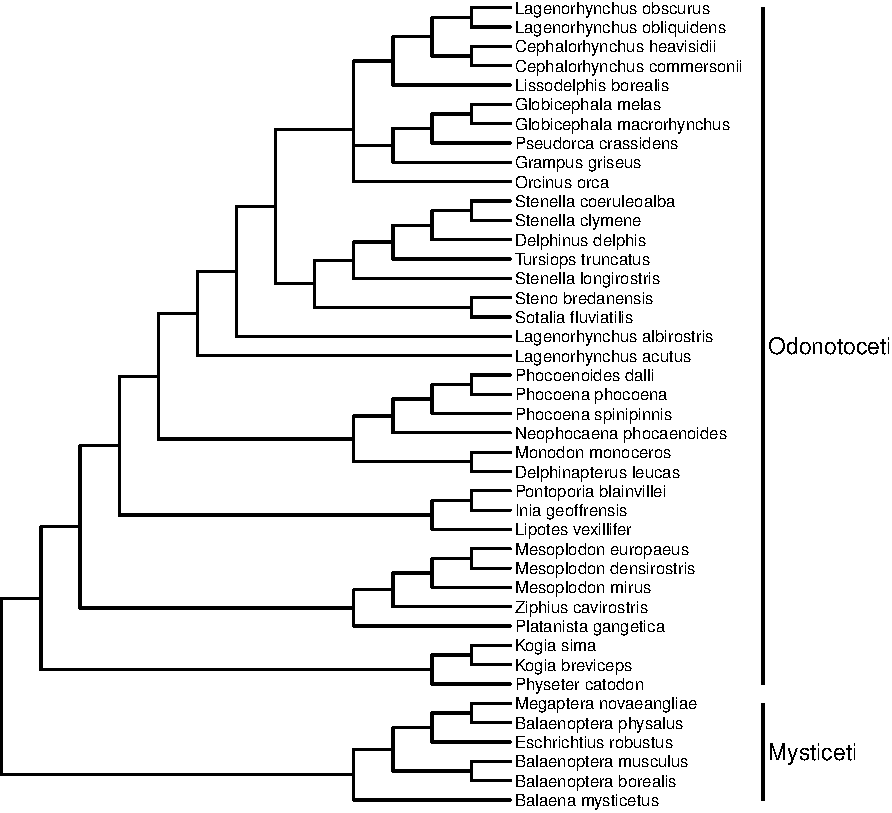
\includegraphics{bookdown-demo_files/figure-latex/unnamed-chunk-4-1.pdf}
\caption{\label{fig:unnamed-chunk-4}A cladogram of 42 cetacean species.}
\end{figure}

The extant species are displayed on the \textbf{tips} of the tree and are connected to each other according to the degree of relatedness by the \textbf{branches}. Figure 2.1 shows us the pattern of relatedness of 42 cetacean species. If we wanted to use these species in a comparative study to investigate the evolutionary history of the group, we would not have independent data points. This means that the assumptions of most statistical tests would be violated and we couldn't trust the results!

This is where phylogenetics comes to the rescue. We can use the pattern of relatedness described by the phylogeny to control for the non-indepedence of data points. To show you what I mean, let's consider body size in those 42 species of cetacean. If we were to show the distribution of body size in the group, we would see that the vast majority of the largest sizes are found in the mysticetes whereas the smaller species tend to be odontocetes. If we viewed these data points as all independent we might say that very large bodies have evolved 7 times in the group (once for each mysticete and once for the sperm whale) whilst small body size has evolved in all the other species (35 times).

In fact, the close relatedness of 6 of the large bodied species suggests that large body size evolved once and not independently for each of these species. Their shared evolutionary history explains why their traits (body size in this case) are so similar. The seventh example of a large body (sperm whales) does not share very much history with the other 6 and this may be of some interest to us. It suggests an independent evolution of large body size and potentially something of interest to us as researchers.

So hopefully you can see how taking phylogeny into account can be illuminating. For a broader (and much more useful) introduction to phylogenetics and its use in evolutionary biology, check out these sources:

\begin{itemize}
\tightlist
\item
  Tree Thinking: An Introduction to Phylogenetic Biology \citep{baum12}
\item
  The Comparative Approach in Evolutionary Anthropology and Biology \citep{Nunn11}
\end{itemize}

\hypertarget{recap}{%
\chapter{R recap}\label{recap}}

In LIFE223, we taught you how to use R for statistical analysis and visualising data. This chapter will contain a basic overview of some of the things from 223 that you may find useful as we proceed. You only need to bother with this if you are new to R or have blocked it from your memory since you last used it.

\hypertarget{basics}{%
\section{Basics}\label{basics}}

R works well as a calculator.

\begin{Shaded}
\begin{Highlighting}[]
\DecValTok{6}\OperatorTok{*}\DecValTok{7}
\end{Highlighting}
\end{Shaded}

\begin{verbatim}
[1] 42
\end{verbatim}

However, R is capable of a great deal more than just simple mathematical operations like multiply and divide. It also has functions that can calculate some common descriptive stats like mean and standard deviation.

\begin{Shaded}
\begin{Highlighting}[]
\KeywordTok{mean}\NormalTok{(x)}
\end{Highlighting}
\end{Shaded}

\begin{verbatim}
[1] 41.97773
\end{verbatim}

\begin{Shaded}
\begin{Highlighting}[]
\KeywordTok{sd}\NormalTok{(x)}
\end{Highlighting}
\end{Shaded}

\begin{verbatim}
[1] 4.185262
\end{verbatim}

\hypertarget{plotting}{%
\subsection{Plotting}\label{plotting}}

R is also a very flexible graphical tool. From LIFE223, you probably remember a few basic plotting functions. Each function in R has arguments that can be added to label axes or change point size as you can see in these plots.

\begin{Shaded}
\begin{Highlighting}[]
\KeywordTok{boxplot}\NormalTok{(x, }\DataTypeTok{ylab =} \StringTok{"Potential answers"}\NormalTok{)}
\end{Highlighting}
\end{Shaded}

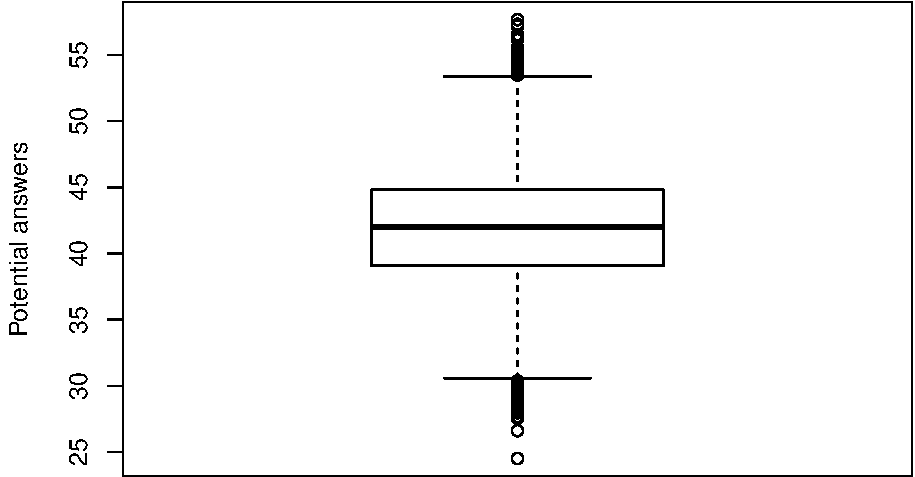
\includegraphics{bookdown-demo_files/figure-latex/unnamed-chunk-9-1.pdf}

\begin{Shaded}
\begin{Highlighting}[]
\KeywordTok{hist}\NormalTok{(x, }\DataTypeTok{xlab =} \StringTok{"Potential answers"}\NormalTok{, }\DataTypeTok{breaks =} \DecValTok{25}\NormalTok{)}
\end{Highlighting}
\end{Shaded}

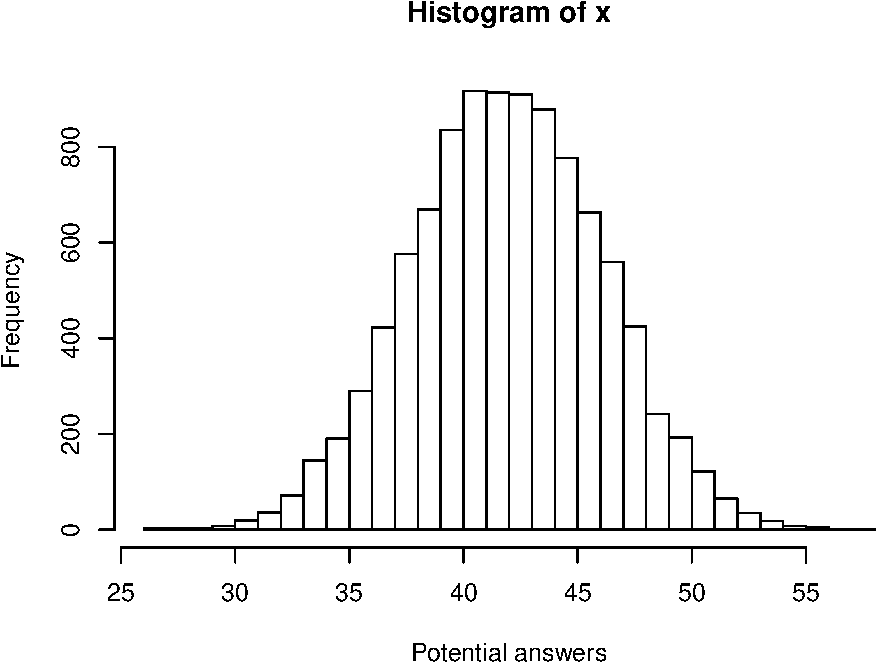
\includegraphics{bookdown-demo_files/figure-latex/unnamed-chunk-9-2.pdf}

\begin{Shaded}
\begin{Highlighting}[]
\KeywordTok{plot}\NormalTok{(x, y, }\DataTypeTok{xlab =} \StringTok{"Potential answers"}\NormalTok{, }\DataTypeTok{pch =} \DecValTok{19}\NormalTok{, }\DataTypeTok{cex =} \FloatTok{0.1}\NormalTok{)}
\end{Highlighting}
\end{Shaded}

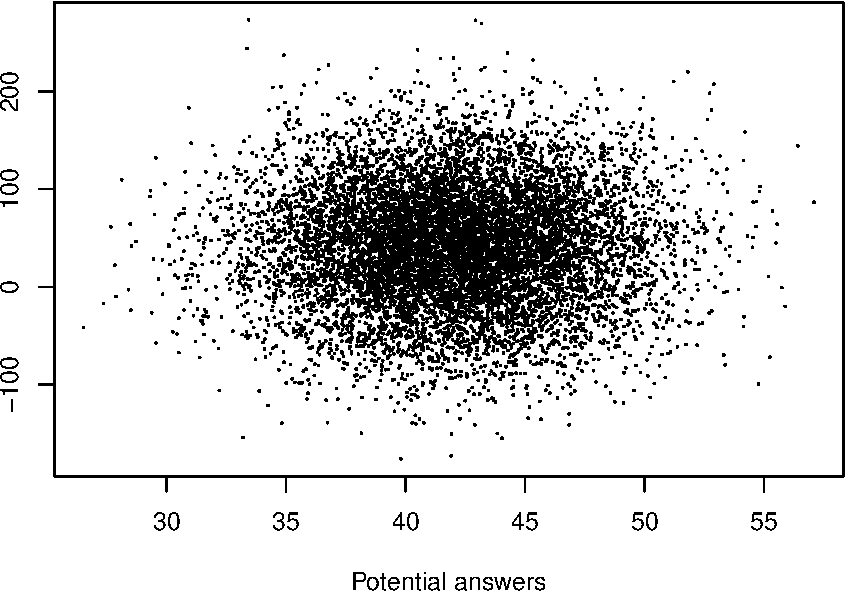
\includegraphics{bookdown-demo_files/figure-latex/unnamed-chunk-9-3.pdf}

For much of this book, I will actually be doing most plotting in a package called \textbf{ggplot2}. This package has a slightly different syntax to get used to but the increased flexibility you have will be a good payoff. Plus the plots look quite nice.

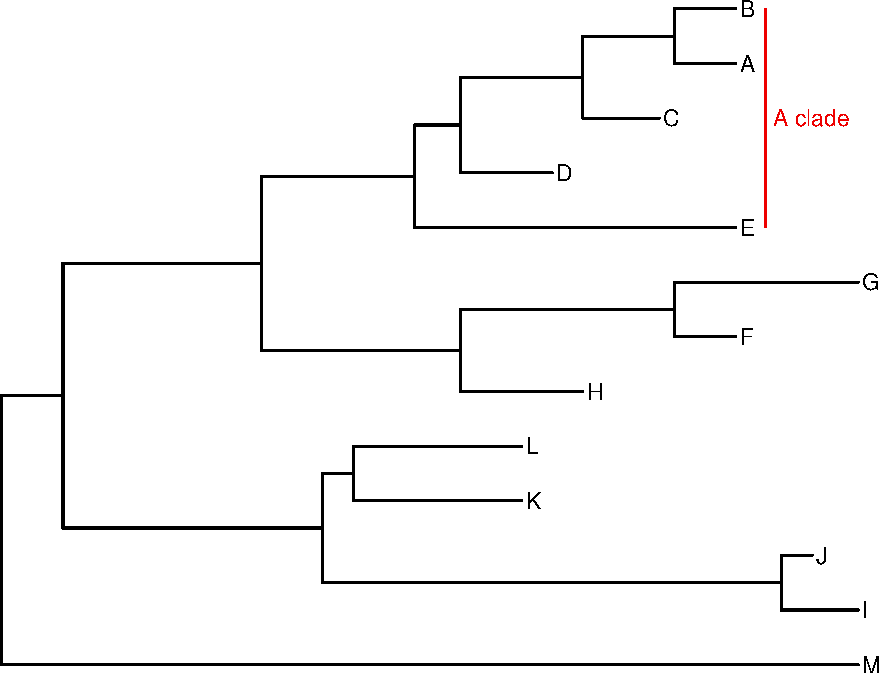
\includegraphics{bookdown-demo_files/figure-latex/unnamed-chunk-10-1.pdf}

\hypertarget{the-working-directory}{%
\subsection{The working directory}\label{the-working-directory}}

The working directory is the folder on your computer where R's attention is focused. This is where you should store any files you need R to open. You can find out the path of the current working directory using the function \textbf{getwd()}

\begin{Shaded}
\begin{Highlighting}[]
\KeywordTok{getwd}\NormalTok{()}
\end{Highlighting}
\end{Shaded}

\begin{verbatim}
[1] "/Users/chrismitchell/Google Drive/University of Liverpool/GitHub Stuff/bookdownCRG"
\end{verbatim}

If this isn't the folder we want as our working directory, we can just as easily change it with \textbf{setwd()}

\begin{Shaded}
\begin{Highlighting}[]
\KeywordTok{setwd}\NormalTok{(}\StringTok{"\textasciitilde{}/Desktop/My R Folder"}\NormalTok{)}
\end{Highlighting}
\end{Shaded}

If you are using RStudio there is also a shortcut to do this in the \emph{Files} pane (usually bottom right). Use this pane to navigate to your chosen directory and then use the drop down menu under \emph{More} (look for a blue cog) to set the current folder as your working directory.

If you aren't using RStudio, I'd strongly suggest you start. It's much more user friendly than base R.

\hypertarget{loading-data}{%
\subsection{Loading data}\label{loading-data}}

Data comes in many forms and R is capable of reading most of them if you know the correct functions. One of the most common formats is \emph{comma separated values}. This has the file extension .csv at the end of the filename. If you open a .csv file with MS Excel or Numbers, you will see that it usually looks much like a spreadsheet. To load a .csv data file into R, use the function \textbf{read.csv()} as shown here.

\begin{Shaded}
\begin{Highlighting}[]
\NormalTok{data \textless{}{-}}\StringTok{ }\KeywordTok{read.csv}\NormalTok{(}\DataTypeTok{file =} \StringTok{"DATAFILE.csv"}\NormalTok{)}
\end{Highlighting}
\end{Shaded}

For other data formats, you may require a different function. For example, data may be provided as a text file (extension .txt). In this case, you need \textbf{read.table()}. Note that with this function you need to specify that your data has a header (a top row with names for columns) whereas \textbf{read.csv()} assumes this by default.

\begin{Shaded}
\begin{Highlighting}[]
\NormalTok{data \textless{}{-}}\StringTok{ }\KeywordTok{read.table}\NormalTok{(}\DataTypeTok{file =} \StringTok{"DATAFILE.txt"}\NormalTok{, }\DataTypeTok{header =} \OtherTok{TRUE}\NormalTok{)}
\end{Highlighting}
\end{Shaded}

\hypertarget{subsetting}{%
\subsection{Subsetting}\label{subsetting}}

Let's say I want to subset my data based on a certain condition. I can achieve this multiple ways but one of the simplest is the function subset.

\begin{Shaded}
\begin{Highlighting}[]
\NormalTok{newdata \textless{}{-}}\StringTok{ }\KeywordTok{subset}\NormalTok{(data, species }\OperatorTok{==}\StringTok{ "Homo sapiens"}\NormalTok{)}
\end{Highlighting}
\end{Shaded}

This function takes a subset of the object \emph{data} and applies the rule that the value of each row in the column \emph{species} be \emph{Homo sapiens}. Thus it extracts the lines of data that are from human beings.

\hypertarget{errors}{%
\section{Errors}\label{errors}}

Error messages are a part of life with R. You are not expected to be able to interpret every single one immediately and you definitely shouldn't panic or give up when you get one.

Here's a basic error message:

\begin{Shaded}
\begin{Highlighting}[]
\NormalTok{data \textless{}{-}}\StringTok{ }\KeywordTok{read.csv}\NormalTok{(}\StringTok{"mydaat.csv"}\NormalTok{)}
\end{Highlighting}
\end{Shaded}

\begin{verbatim}
Warning in file(file, "rt"): cannot open file 'mydaat.csv': No such file or
directory
\end{verbatim}

\begin{verbatim}
Error in file(file, "rt"): cannot open the connection
\end{verbatim}

The message tells me that R ``cannot open the connection'' and no such file exists. This means that R cannot find the file I was looking for in the current working directory. It could be because I haven't set the correct working directory or the file is there but in a different format. In this case, the error has appeared because I have spelled the name incorrectly. I have sent R looking for a file called \emph{mydaat.csv} instead of \emph{mydata.csv}. Always remember that R is a useful idiot and will only do exactly what you tell it to do!

\hypertarget{google}{%
\section{Google}\label{google}}

The most important skill you need for using R is the ability to use Google (other search engines are available). It may seem odd but almost any problem you will ever encounter with R can be solved by a quick Google search.

If you come up against a confusing error message, copy and paste the message into Google. You will quickly land on one of the forums where someone else has asked about the same error message. The odds are pretty good you'll discover an explanation for the problem there.

If you don't know how to do something, pop the name of what you want to do into Google and add ``in R'' at the end and there will almost always be a tutorial on the first page of results with exactly what you need.

Seriously, Google is your strongest ally here. The community of R users has populated the internet with endless advice and guidance for every level from beginner to the most advanced of users. That brings me to my next point\ldots{}

\hypertarget{stealing}{%
\section{Stealing}\label{stealing}}

If imitation is the greatest form of flattery then learning to code in R is just about the most flattering thing you can do. The internet is teeming with examples of R code for all kinds of purposes including in this very book. Take it without thinking twice.

You will have acheived a pretty good level of skill in R when you can take someone else's code and edit it for your own purposes. This is the \textbf{core skill} of R and once you can do that, you'll be unstoppable.

\hypertarget{phylogenetics}{%
\chapter{Phylogenetic trees and where to find them}\label{phylogenetics}}

This chapter is a brief overview of some key concepts that may be useful when performing comparative research.

\hypertarget{phylogeny}{%
\section{Phylogeny}\label{phylogeny}}

Phylogeny is the term used to describe the evolutionary history of a group of species. The most common representation of phylogeny is a phylogenetic tree. There is a lot of terminology around phylogenetic trees. Here we will start with the very basics that will come up a lot in this book.

The \textbf{tips} of the tree represent the species/populations/individuals described by the tree. The \textbf{branches} of the tree represent the pattern of relationships between species. The \textbf{nodes} of a tree represent the most recent common ancestor of the lineages that diverge from that node. A \textbf{clade} is a monophyletic grouping of lineages. A grouping is \textbf{monophyletic} only if all members of that group descend from a common ancestor to the exclusion of others. for example, humans and apes form a monophyletic grouping but humans, apes and parrots do not.

Here is an example of a phylogenetic tree displaying the relationships of modern dog breeds taken from a nice paper investigating the evolutionary history of the domestic dog \citep{Parker17}

The tree shown above is a \textbf{cladogram} meaning that the lengths of the branches do not carry any real meaning. This tree is only useful for interpreting the relatedness of the species. It does not give us any information about the amount of evolutionary change or the amount time between nodes.

By contrast, the following tree has \textbf{branch lengths}. The tree is based on genetic analysis of 173 species of hymenoptera (bees, ants and wasps) \citep{Peters17}. In this tree, the branch lengths represent time (in millions of years) as calculated from analysis of over 3,000 genes and calibrated using fossils.

Branch lengths do not always represent evolutionary distance as time. In some cases, evolutionary distance is represented as the amount of change on each branch. The next tree was built based on a brain development gene (MCPH1) in cetaceans (whales, dolphins and porpoises) \citep{McGowen11}. On a tree like this, longer branches indicate more character changes along the branch. In this case the character changes will be changes in genetic sequence but for other trees it may be morphological characters, protein sequences characters or a combination.

\hypertarget{building-trees}{%
\section{Building trees}\label{building-trees}}

Developments in the field of phylogenetics have meant that there are many ways to construct a phylogeny. Many of the modern methods are highly sophistaicated and for now, these are not the subject of this book. However, it may help you to have a brief introduction to the logic behind building a phylogeny.

\hypertarget{locating-trees}{%
\section{Locating trees}\label{locating-trees}}

\hypertarget{file-format}{%
\subsection{File format}\label{file-format}}

\hypertarget{w1plotting}{%
\chapter{Plotting trees in R}\label{w1plotting}}

\hypertarget{phylogenies-in-r}{%
\section{Phylogenies in R}\label{phylogenies-in-r}}

From LIFE223, you know R as a powerful statistical tool. You will also be aware that it is an incredibly flexible tool for plotting data. In this workshop, we will be working with phylogenies in R and manipulating them to produce informative plots.

\hypertarget{packages-used}{%
\subsection{Packages used}\label{packages-used}}

In this section we'll mostly be using a package called ggtree \citep{Yu17, Yu18}. To install it, we need another package called \textbf{BiocManager} \citep{Morgan19}.

\begin{Shaded}
\begin{Highlighting}[]
\KeywordTok{install.packages}\NormalTok{(}\StringTok{"BiocManager"}\NormalTok{)}
\NormalTok{BiocManager}\OperatorTok{::}\KeywordTok{install}\NormalTok{(}\StringTok{"ggtree"}\NormalTok{)}
\KeywordTok{library}\NormalTok{(ggtree)}
\end{Highlighting}
\end{Shaded}

\begin{Shaded}
\begin{Highlighting}[]
\KeywordTok{library}\NormalTok{(ggtree)}
\end{Highlighting}
\end{Shaded}

We will also need to use phylobase \citep{phylobase}, ggimage \citep{Yu19} and it would help to have the tidyverse packages loaded \citep{Wickham17} since we'll be using the syntax of ggplot2. If you get an error message, make sure the packages are installed first.

\begin{Shaded}
\begin{Highlighting}[]
\KeywordTok{library}\NormalTok{(tidyverse)}
\KeywordTok{library}\NormalTok{(phylobase)}
\KeywordTok{library}\NormalTok{(ggimage)}
\end{Highlighting}
\end{Shaded}

\hypertarget{importing-your-tree}{%
\section{Importing your tree}\label{importing-your-tree}}

Let's start by importing a tree. Make sure your working directory is set to wherever you have saved the tree\_newick file. If you run this line, you should see an object called ``tree'' appear in your global environment.

\begin{Shaded}
\begin{Highlighting}[]
\NormalTok{tree \textless{}{-}}\StringTok{ }\KeywordTok{read.tree}\NormalTok{(}\StringTok{"tree\_newick.nwk"}\NormalTok{)}
\end{Highlighting}
\end{Shaded}

If we take a look at the structure of our tree object using the \textbf{str} function we can see that the tree is stored as an object of class \textbf{phylo}. If you are using a block of trees (more on this subsequent chapters) it will be an object of class \textbf{multiphylo}.

\begin{Shaded}
\begin{Highlighting}[]
\KeywordTok{str}\NormalTok{(tree)}
\end{Highlighting}
\end{Shaded}

\begin{verbatim}
List of 4
 $ edge       : int [1:24, 1:2] 14 15 16 17 18 19 20 20 19 18 ...
 $ edge.length: num [1:24] 4 13 10 3 8 6 4 4 5 6 ...
 $ Nnode      : int 12
 $ tip.label  : chr [1:13] "A" "B" "C" "D" ...
 - attr(*, "class")= chr "phylo"
 - attr(*, "order")= chr "cladewise"
\end{verbatim}

We can see a list of 4 elements of the tree object. The first (\textbf{edge}) contains the edges (also known as branches) of the phylogeny and their labels. The next is \textbf{edge.length} which contains the lengths of the branches if present (see \textbf{chapter 3} for more details). \textbf{Nnode} specifies the number of nodes and finally \textbf{tip.label} contains the labels of the tips. In this case, we just have letters for tip labels.

Things are often clearer when we plot them. We can do this for trees with the \textbf{plot} function in base R. This function is incredibly versatile and you should recognise it from LIFE223. Here we are using very different arguments.

\begin{Shaded}
\begin{Highlighting}[]
\KeywordTok{plot}\NormalTok{(tree)}
\end{Highlighting}
\end{Shaded}

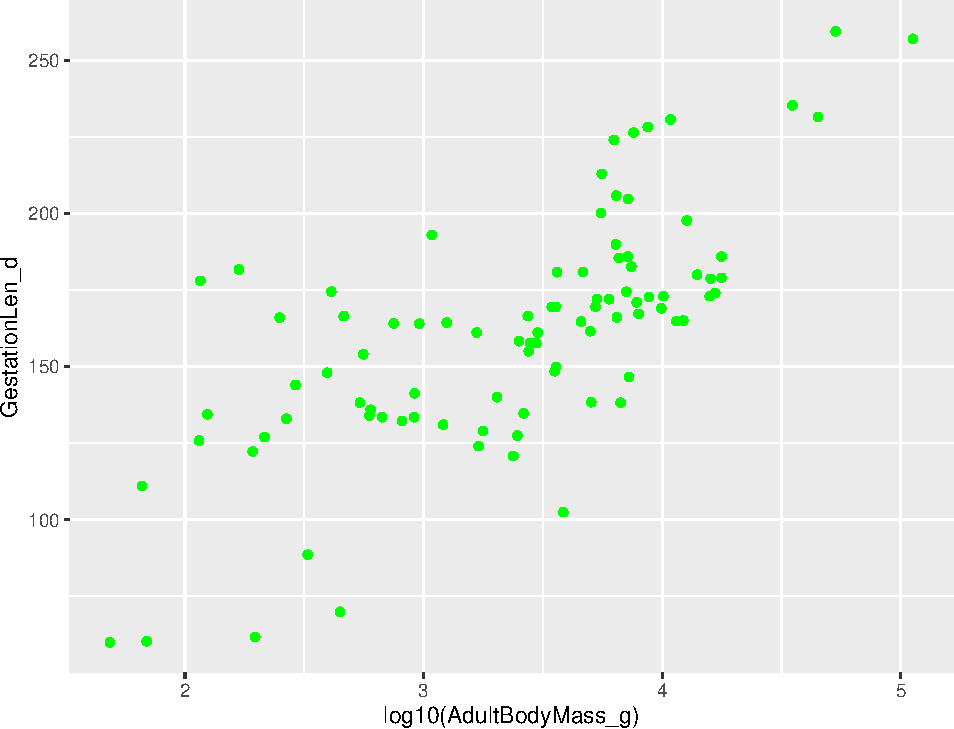
\includegraphics{bookdown-demo_files/figure-latex/unnamed-chunk-28-1.pdf}

This plot is fine for a quick check to make sure the tree looks as we expected it to. Let's look at making a more attractive plot with ggtree.

\hypertarget{ggtree}{%
\section{ggtree}\label{ggtree}}

The package ggtree is an extension of \textbf{ggplot2}, a popular plotting package from the \textbf{tidyverse} family of packages. The syntax we'll be using here is a little different that what you may be used to so don't get intimidated. \textbf{ggtree} uses the same syntax as \textbf{ggplot2}. This works by creating layers (known as \textbf{geoms}) and plotting them over each other to build up the plot.

We'll start by using ggtree to plot our tree. Below is the base layer of the plot. There are many other options we can include to customise our tree. Try some out in this R window to see how they effect your plot.

\hypertarget{geoms}{%
\subsection{Geoms}\label{geoms}}

Geoms are new layers to plot on or alongside your tree. Now let's try plotting it whilst adding new layers. These geoms can be combined as you see fit. This gives you a lot of flexibility in how you plot your trees. For example, we can add a geom to include the tip labels for our tree.

\begin{Shaded}
\begin{Highlighting}[]
\KeywordTok{ggtree}\NormalTok{(tree) }\OperatorTok{+}\StringTok{ }
\StringTok{  }\KeywordTok{geom\_tiplab}\NormalTok{()}
\end{Highlighting}
\end{Shaded}

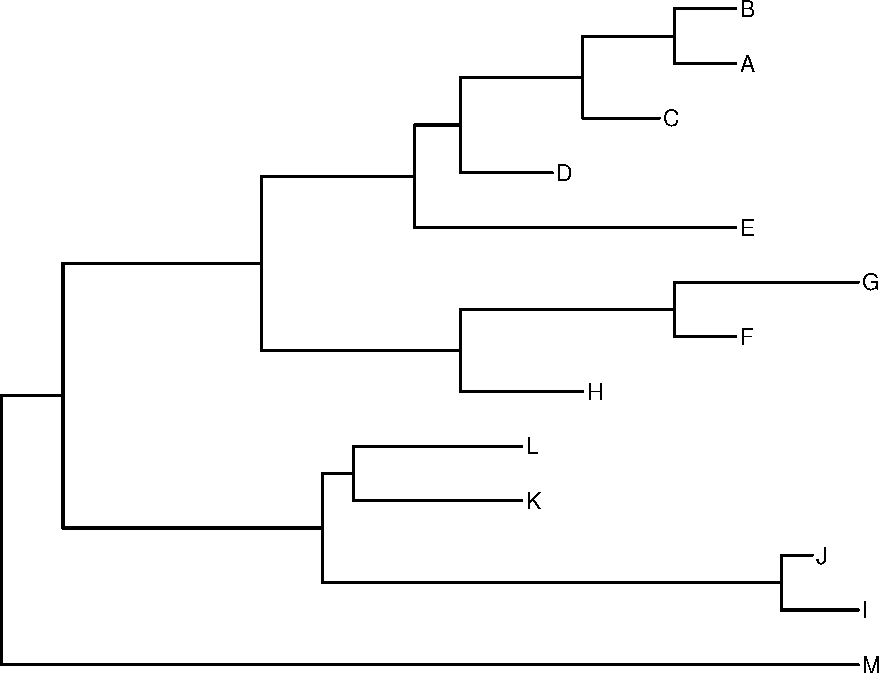
\includegraphics{bookdown-demo_files/figure-latex/unnamed-chunk-29-1.pdf}

And we can add a title

\begin{Shaded}
\begin{Highlighting}[]
\KeywordTok{ggtree}\NormalTok{(tree) }\OperatorTok{+}\StringTok{ }
\StringTok{  }\KeywordTok{geom\_tiplab}\NormalTok{() }\OperatorTok{+}
\StringTok{  }\KeywordTok{ggtitle}\NormalTok{(}\StringTok{"A phylogeny of letters. For some reason..."}\NormalTok{)}
\end{Highlighting}
\end{Shaded}

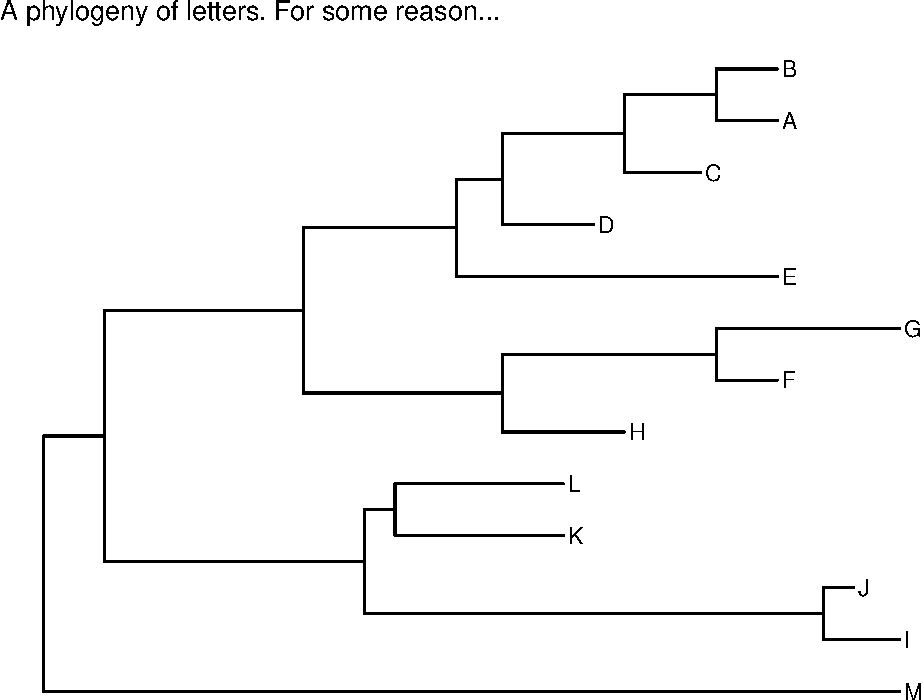
\includegraphics{bookdown-demo_files/figure-latex/unnamed-chunk-30-1.pdf}

There are many geoms you can use to add more information to your plot. Here are just a few that you may want to investigate.

\begin{Shaded}
\begin{Highlighting}[]
\KeywordTok{geom\_tiplab}\NormalTok{() }\CommentTok{\#adds tiplables}
\KeywordTok{geom\_tippoint}\NormalTok{() }\CommentTok{\#adds points at the tips}
\KeywordTok{geom\_nodepoint}\NormalTok{() }\CommentTok{\#adds points at the nodes}
\KeywordTok{geom\_nodelab}\NormalTok{() }\CommentTok{\#adds labels for nodes}
\KeywordTok{geom\_cladelabel}\NormalTok{() }\CommentTok{\#adds labels for clades}
\end{Highlighting}
\end{Shaded}

\hypertarget{labelling-clades}{%
\subsection{Labelling clades}\label{labelling-clades}}

As an example of what you might like to do with ggtree, let's have a look at adding some labels to identify some clades on our tree. To label clades, we need to be able to identify the node of the most recent common ancestor. The function \textbf{MRCA} in the package \textbf{phylobase} \citep{phylobase} tells us that the common ancestor of C and E is node 17.

\begin{Shaded}
\begin{Highlighting}[]
\NormalTok{phylobase}\OperatorTok{::}\KeywordTok{MRCA}\NormalTok{(tree, }\DataTypeTok{tip =} \KeywordTok{c}\NormalTok{(}\StringTok{"C"}\NormalTok{, }\StringTok{"E"}\NormalTok{))}
\end{Highlighting}
\end{Shaded}

\begin{verbatim}
[1] 17
\end{verbatim}

We can now use the \textbf{geom\_cladelabel} geom to add a simple label for the clade descended from the appropriate node. Take note of the arguments I've added to customise the geom. You may want to play around with these options yourself to see how they work.

\begin{Shaded}
\begin{Highlighting}[]
\KeywordTok{ggtree}\NormalTok{(tree) }\OperatorTok{+}\StringTok{ }
\StringTok{  }\KeywordTok{geom\_tiplab}\NormalTok{() }\OperatorTok{+}\StringTok{ }
\StringTok{  }\KeywordTok{geom\_cladelabel}\NormalTok{(}\DataTypeTok{node=}\DecValTok{17}\NormalTok{, }\DataTypeTok{label=}\StringTok{"A clade"}\NormalTok{, }
                  \DataTypeTok{color=}\StringTok{"red2"}\NormalTok{, }\DataTypeTok{offset=}\DecValTok{1}\NormalTok{)}
\end{Highlighting}
\end{Shaded}

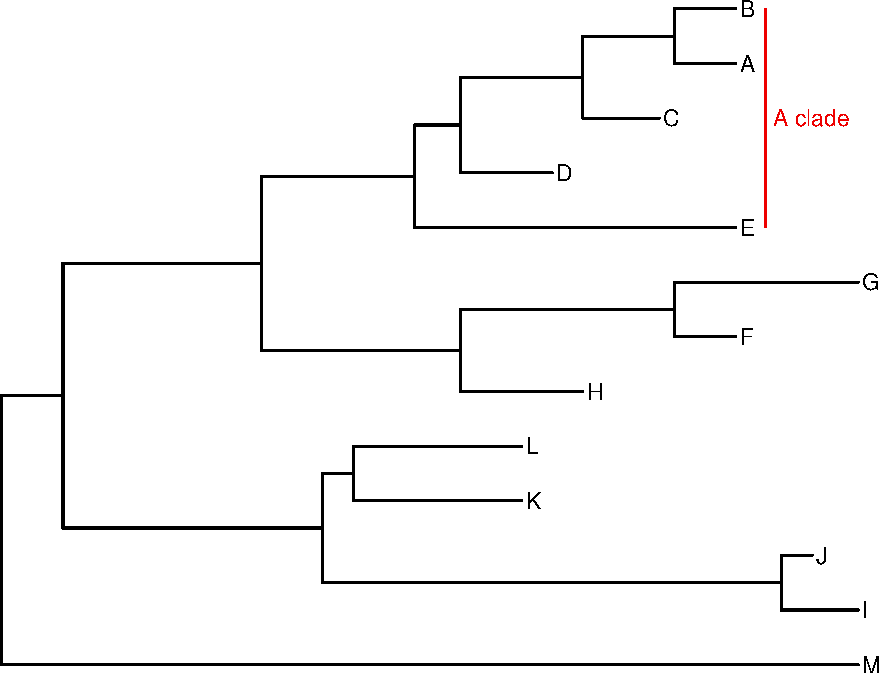
\includegraphics{bookdown-demo_files/figure-latex/unnamed-chunk-33-1.pdf}

Pretty good but there are other options. This is a matter of personal preference. You may prefer to overlay a translucent rectangle over your clade of interest.

\begin{Shaded}
\begin{Highlighting}[]
\KeywordTok{ggtree}\NormalTok{(tree) }\OperatorTok{+}\StringTok{ }
\StringTok{  }\KeywordTok{geom\_tiplab}\NormalTok{() }\OperatorTok{+}\StringTok{ }
\StringTok{  }\KeywordTok{geom\_hilight}\NormalTok{(}\DataTypeTok{node=}\DecValTok{17}\NormalTok{, }\DataTypeTok{fill=}\StringTok{"gold"}\NormalTok{)}
\end{Highlighting}
\end{Shaded}

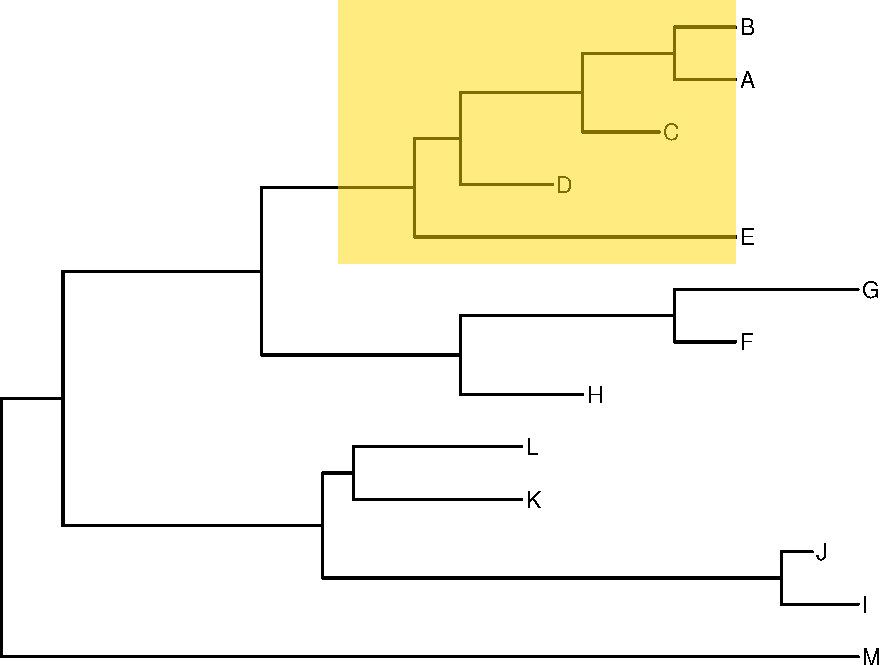
\includegraphics{bookdown-demo_files/figure-latex/unnamed-chunk-34-1.pdf}

Use the R window below to experiment with the available geoms in ggtree. Find a combination that suits you and your tree.

\hypertarget{adding-images-to-trees}{%
\section{Adding images to trees}\label{adding-images-to-trees}}

As you probably noted in chapter 3, adding images to a plot is an excellent way to annotate your tree. The ggtree package can do this as you can see here.

\begin{figure}
\centering
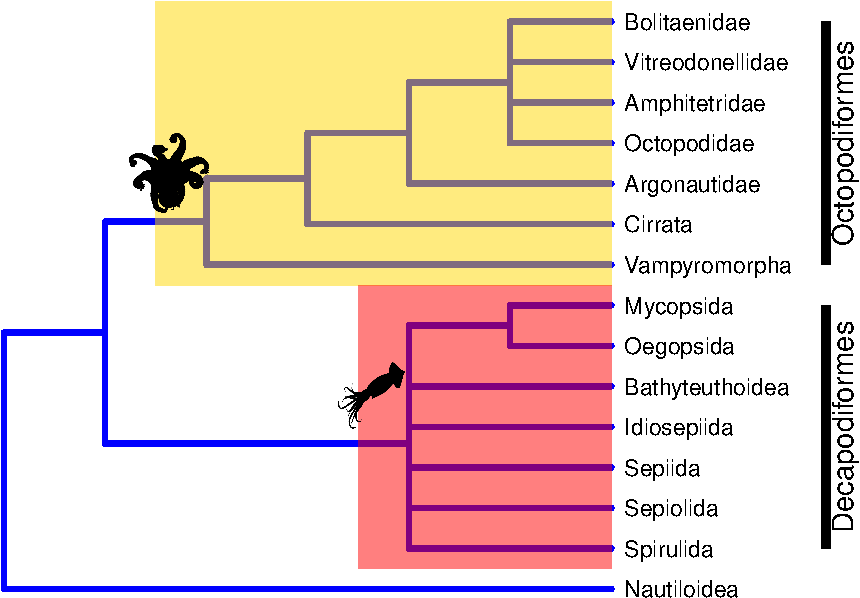
\includegraphics{bookdown-demo_files/figure-latex/unnamed-chunk-35-1.pdf}
\caption{\label{fig:unnamed-chunk-35}Plot of cephalopod families annotated using ggtree and Phylopic.}
\end{figure}

This phylogeny is annotated in a number of useful ways. The tip labels describe cephalopod families. The superorders (octopodiformes and decapodiformes) are highlighted by gold and red rectangles as well as a bar across the tips. this demonstrates how multiple geoms can combine to make a plot easy to interpret.

The most interesting thing for our purposes are the silhouettes at the root of each superorder. The octopodiformes have an octopus and the decapodiformes have a squid as example taxa from within the superorder.

\hypertarget{phylopic}{%
\subsection{Phylopic}\label{phylopic}}

The silhouettes used for that plot are from a website called \href{http://phylopic.org/}{Phylopic}. Phylopic provides open source biological silhouettes that are free to use. We're now going to look at how to get these silhouettes and use them to annotate our trees.

Let's start with loading an example tree. This one is a primate tree courtesy of \href{https://www.randigriffin.com/}{Randi Griffin}. You'll notice that I'm loading this tree using a url. This is because I'm loading a file directly from GitHub, a repository for all sorts of code and the host of this site! Randi (and many other coders) make some of the things they produce freely available through GitHub. This can be data, files or code.

\begin{Shaded}
\begin{Highlighting}[]
\NormalTok{primates \textless{}{-}}\StringTok{ }\KeywordTok{read.nexus}\NormalTok{(}\StringTok{"https://raw.githubusercontent.com/rgriff23/Dissertation/master/Chapter\_2/data/tree.nex"}\NormalTok{)}
\end{Highlighting}
\end{Shaded}

Let's plot the new tree first. Here I'm assigning the plot to a named object (p1) in R. This means that instead of immediately printing out the plot, R stores it in the working directory. The reason for doing this will become clear as we go on. It saves us typing out every line of code each time we want to add a new geom!

\begin{Shaded}
\begin{Highlighting}[]
\NormalTok{p1 \textless{}{-}}\StringTok{ }\KeywordTok{ggtree}\NormalTok{(primates)}
\NormalTok{p1}
\end{Highlighting}
\end{Shaded}

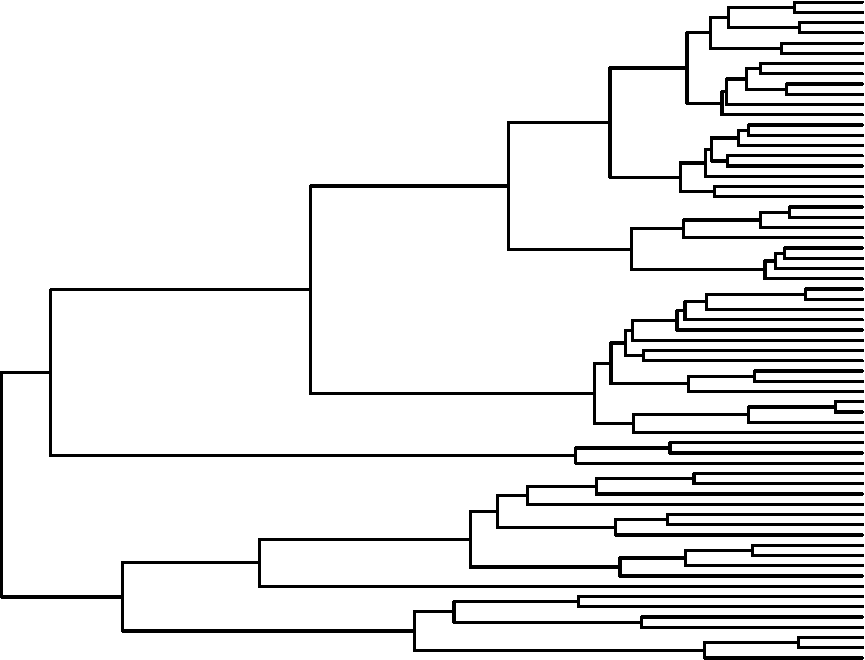
\includegraphics{bookdown-demo_files/figure-latex/unnamed-chunk-38-1.pdf}

Let's use what we already know about ggtree to customise this plot into something more useful. In particular, this plot is quite useful because it tells us the numbers of each node and we will need that later on.

\begin{Shaded}
\begin{Highlighting}[]
\KeywordTok{ggtree}\NormalTok{(primates) }\OperatorTok{+}
\StringTok{   }\KeywordTok{xlim}\NormalTok{(}\DecValTok{0}\NormalTok{,}\DecValTok{90}\NormalTok{) }\OperatorTok{+}\StringTok{ }
\StringTok{   }\KeywordTok{geom\_tiplab}\NormalTok{(}\DataTypeTok{size=}\FloatTok{1.5}\NormalTok{) }\OperatorTok{+}
\StringTok{   }\KeywordTok{geom\_label2}\NormalTok{(}\KeywordTok{aes}\NormalTok{(}\DataTypeTok{subset=}\OperatorTok{!}\NormalTok{isTip, }\DataTypeTok{label=}\NormalTok{node), }\DataTypeTok{size=}\DecValTok{2}\NormalTok{, }\DataTypeTok{color=}\StringTok{"darkred"}\NormalTok{, }\DataTypeTok{alpha=}\FloatTok{0.5}\NormalTok{)}
\end{Highlighting}
\end{Shaded}

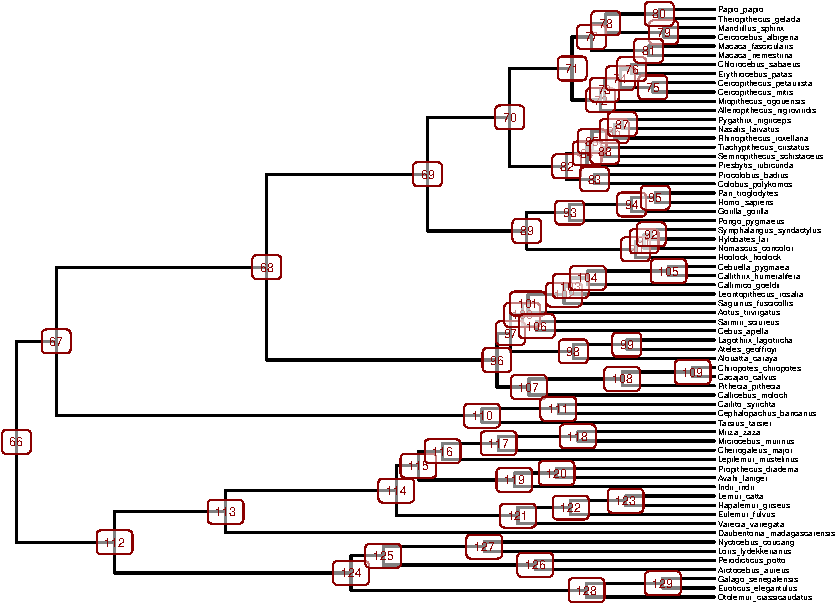
\includegraphics{bookdown-demo_files/figure-latex/unnamed-chunk-39-1.pdf}

Let's label the 6 primate superfamilies using the node numbers I have extracted from the previous plot. You can choose whatever colours you prefer here. I've also added some useful features to this code. the use of \textbf{xlim()} can be very useful when plotting a tree with some extra space for more details. Here I've set the limits of the x dimension (the horizontal) to be between 0 and 100. This gives me space for later annotations.

\begin{Shaded}
\begin{Highlighting}[]
\NormalTok{p2 \textless{}{-}}\StringTok{ }\KeywordTok{ggtree}\NormalTok{(primates) }\OperatorTok{+}
\StringTok{  }\KeywordTok{xlim}\NormalTok{(}\DecValTok{0}\NormalTok{,}\DecValTok{100}\NormalTok{) }\OperatorTok{+}
\StringTok{  }\KeywordTok{geom\_tiplab}\NormalTok{(}\DataTypeTok{size=}\FloatTok{1.5}\NormalTok{, }\DataTypeTok{offset=}\FloatTok{0.5}\NormalTok{) }\OperatorTok{+}
\StringTok{  }\KeywordTok{geom\_hilight}\NormalTok{(}\DataTypeTok{node=}\DecValTok{124}\NormalTok{, }\DataTypeTok{fill=}\StringTok{"steelblue"}\NormalTok{, }\DataTypeTok{alpha=}\FloatTok{0.5}\NormalTok{) }\OperatorTok{+}
\StringTok{  }\KeywordTok{geom\_hilight}\NormalTok{(}\DataTypeTok{node=}\DecValTok{113}\NormalTok{, }\DataTypeTok{fill=}\StringTok{"darkgreen"}\NormalTok{, }\DataTypeTok{alpha=}\FloatTok{0.5}\NormalTok{) }\OperatorTok{+}
\StringTok{  }\KeywordTok{geom\_hilight}\NormalTok{(}\DataTypeTok{node=}\DecValTok{110}\NormalTok{, }\DataTypeTok{fill=}\StringTok{"gray"}\NormalTok{, }\DataTypeTok{alpha=}\FloatTok{0.5}\NormalTok{) }\OperatorTok{+}
\StringTok{  }\KeywordTok{geom\_hilight}\NormalTok{(}\DataTypeTok{node=}\DecValTok{96}\NormalTok{, }\DataTypeTok{fill=}\StringTok{"pink"}\NormalTok{, }\DataTypeTok{alpha=}\FloatTok{0.5}\NormalTok{) }\OperatorTok{+}
\StringTok{  }\KeywordTok{geom\_hilight}\NormalTok{(}\DataTypeTok{node=}\DecValTok{89}\NormalTok{, }\DataTypeTok{fill=}\StringTok{"beige"}\NormalTok{, }\DataTypeTok{alpha=}\FloatTok{0.5}\NormalTok{) }\OperatorTok{+}
\StringTok{  }\KeywordTok{geom\_hilight}\NormalTok{(}\DataTypeTok{node=}\DecValTok{70}\NormalTok{, }\DataTypeTok{fill=}\StringTok{"yellow"}\NormalTok{, }\DataTypeTok{alpha=}\FloatTok{0.5}\NormalTok{) }
\NormalTok{p2}
\end{Highlighting}
\end{Shaded}

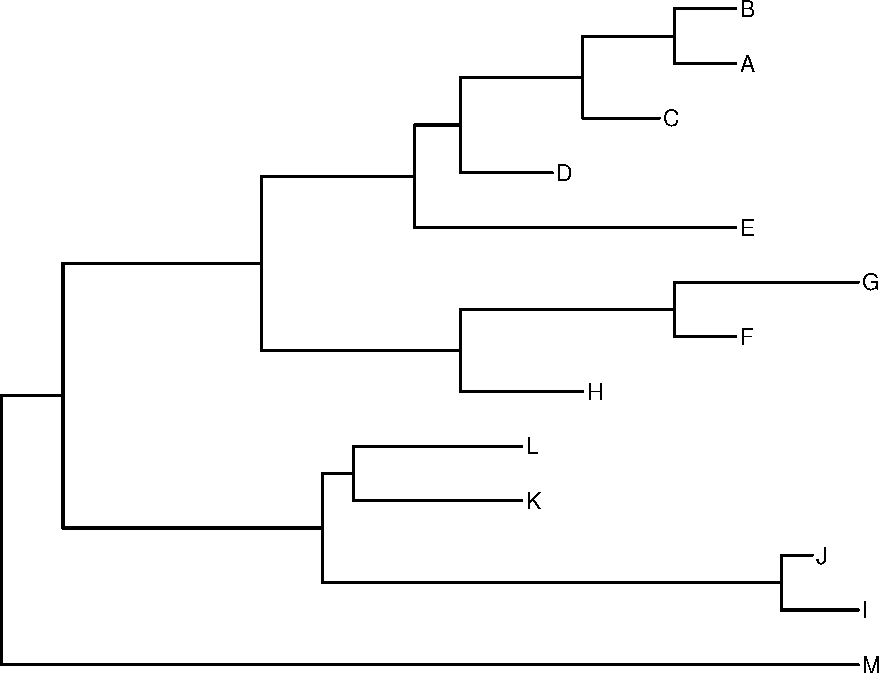
\includegraphics{bookdown-demo_files/figure-latex/unnamed-chunk-40-1.pdf}

So far so good. Let's add on bars to label the superfamilies like I did for the cephalopod version. This time, I'll add the new details to the object p3 to save retyping. Take note of the arguments in each label. You may need to twist these with some trial-and-error to make sure they suit your plot window.

\begin{Shaded}
\begin{Highlighting}[]
\NormalTok{p3 \textless{}{-}}\StringTok{ }\NormalTok{p2 }\OperatorTok{+}
\StringTok{  }\KeywordTok{geom\_cladelabel}\NormalTok{(}\DecValTok{124}\NormalTok{, }\StringTok{"Galagoidea"}\NormalTok{, }\DataTypeTok{offset=}\DecValTok{15}\NormalTok{, }\DataTypeTok{barsize=}\DecValTok{2}\NormalTok{, }\DataTypeTok{angle=}\DecValTok{90}\NormalTok{,}
                  \DataTypeTok{offset.text=}\FloatTok{1.5}\NormalTok{, }\DataTypeTok{hjust=}\FloatTok{0.5}\NormalTok{, }\DataTypeTok{fontsize=}\DecValTok{3}\NormalTok{) }\OperatorTok{+}\StringTok{ }
\StringTok{  }\KeywordTok{geom\_cladelabel}\NormalTok{(}\DecValTok{113}\NormalTok{, }\StringTok{"Lemuroidea"}\NormalTok{, }\DataTypeTok{offset=}\DecValTok{15}\NormalTok{, }\DataTypeTok{barsize=}\DecValTok{2}\NormalTok{, }\DataTypeTok{angle=}\DecValTok{90}\NormalTok{,}
                  \DataTypeTok{offset.text=}\FloatTok{1.5}\NormalTok{, }\DataTypeTok{hjust=}\FloatTok{0.5}\NormalTok{, }\DataTypeTok{fontsize=}\DecValTok{3}\NormalTok{) }\OperatorTok{+}
\StringTok{  }\KeywordTok{geom\_cladelabel}\NormalTok{(}\DecValTok{110}\NormalTok{, }\StringTok{"Tarsioidea"}\NormalTok{, }\DataTypeTok{offset=}\DecValTok{15}\NormalTok{, }\DataTypeTok{barsize=}\DecValTok{2}\NormalTok{, }\DataTypeTok{angle=}\DecValTok{75}\NormalTok{,}
                  \DataTypeTok{offset.text=}\FloatTok{2.5}\NormalTok{, }\DataTypeTok{hjust=}\FloatTok{0.2}\NormalTok{, }\DataTypeTok{fontsize=}\DecValTok{2}\NormalTok{) }\OperatorTok{+}
\StringTok{  }\KeywordTok{geom\_cladelabel}\NormalTok{(}\DecValTok{96}\NormalTok{, }\StringTok{"Ceboidea"}\NormalTok{, }\DataTypeTok{offset=}\DecValTok{15}\NormalTok{, }\DataTypeTok{barsize=}\DecValTok{2}\NormalTok{, }\DataTypeTok{angle=}\DecValTok{90}\NormalTok{,}
                  \DataTypeTok{offset.text=}\FloatTok{1.5}\NormalTok{, }\DataTypeTok{hjust=}\FloatTok{0.5}\NormalTok{, }\DataTypeTok{fontsize=}\DecValTok{3}\NormalTok{) }\OperatorTok{+}
\StringTok{  }\KeywordTok{geom\_cladelabel}\NormalTok{(}\DecValTok{89}\NormalTok{, }\StringTok{"Hominoidea"}\NormalTok{, }\DataTypeTok{offset=}\DecValTok{15}\NormalTok{, }\DataTypeTok{barsize=}\DecValTok{2}\NormalTok{, }\DataTypeTok{angle=}\DecValTok{90}\NormalTok{,}
                  \DataTypeTok{offset.text=}\FloatTok{1.5}\NormalTok{, }\DataTypeTok{hjust=}\FloatTok{0.5}\NormalTok{, }\DataTypeTok{fontsize=}\DecValTok{3}\NormalTok{) }\OperatorTok{+}
\StringTok{  }\KeywordTok{geom\_cladelabel}\NormalTok{(}\DecValTok{70}\NormalTok{, }\StringTok{"Cercopithecoidea"}\NormalTok{, }\DataTypeTok{offset=}\DecValTok{15}\NormalTok{, }\DataTypeTok{barsize=}\DecValTok{2}\NormalTok{, }\DataTypeTok{angle=}\DecValTok{90}\NormalTok{,}
                  \DataTypeTok{offset.text=}\FloatTok{1.5}\NormalTok{, }\DataTypeTok{hjust=}\FloatTok{0.5}\NormalTok{, }\DataTypeTok{fontsize=}\DecValTok{3}\NormalTok{)}
\NormalTok{p3}
\end{Highlighting}
\end{Shaded}

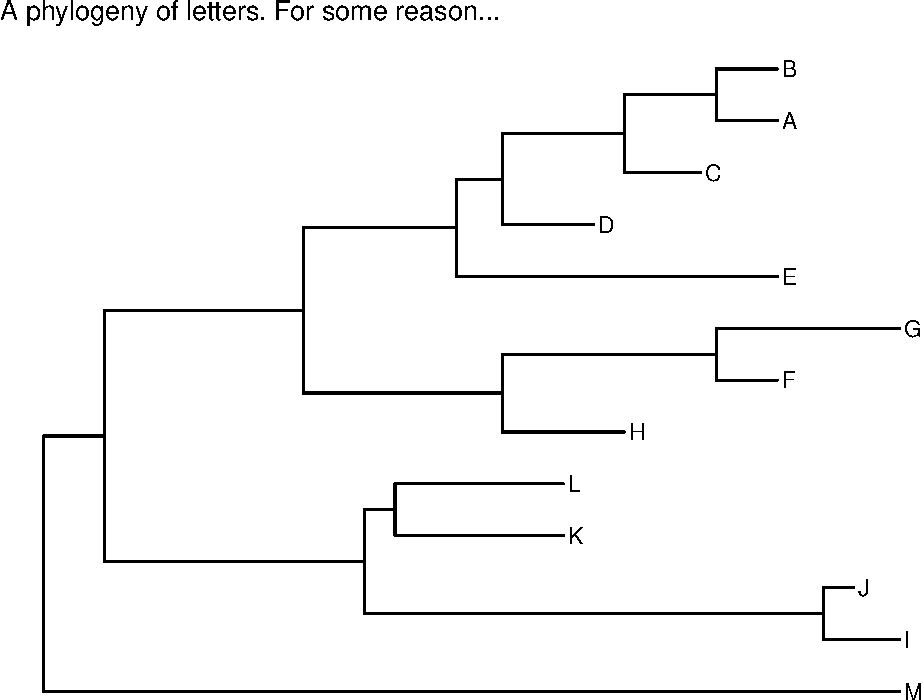
\includegraphics{bookdown-demo_files/figure-latex/unnamed-chunk-41-1.pdf}

There are some helpful details here, such as the fact that the label for Tarsioidea is off at an angle to avoid overlapping with other labels (\emph{angle = 75}). The extra arguments in these options demonstrate how much control you can exercise over each geom.

Now let's get to adding images. The way to do this is a little awkward but I think it's worth the hassle. The first thing we have to do is gather the links for each image we want to use. I've chosen to do this by building a small data frame containing the urls to the images on phylopic, the names of the super families I want to label and the nodes I want to plot the images on.

\begin{Shaded}
\begin{Highlighting}[]
\NormalTok{images \textless{}{-}}\StringTok{ }\KeywordTok{data.frame}\NormalTok{(}\DataTypeTok{node =} \KeywordTok{c}\NormalTok{(}\DecValTok{124}\NormalTok{,}\DecValTok{113}\NormalTok{,}\DecValTok{110}\NormalTok{,}\DecValTok{96}\NormalTok{,}\DecValTok{89}\NormalTok{,}\DecValTok{70}\NormalTok{),}
\DataTypeTok{phylopic =} \KeywordTok{c}\NormalTok{(}\StringTok{"http://phylopic.org/assets/images/submissions/}
\StringTok{7fb9bea8{-}e758{-}4986{-}afb2{-}95a2c3bf983d.512.png"}\NormalTok{,}
\StringTok{"http://phylopic.org/assets/images/submissions/}
\StringTok{bac25f49{-}97a4{-}4aec{-}beb6{-}f542158ebd23.512.png"}\NormalTok{,}
\StringTok{"http://phylopic.org/assets/images/submissions/}
\StringTok{f598fb39{-}facf{-}43ea{-}a576{-}1861304b2fe4.512.png"}\NormalTok{,}
\StringTok{"http://phylopic.org/assets/images/submissions/}
\StringTok{aceb287d{-}84cf{-}46f1{-}868c{-}4797c4ac54a8.512.png"}\NormalTok{,}
\StringTok{"http://phylopic.org/assets/images/submissions/}
\StringTok{0174801d{-}15a6{-}4668{-}bfe0{-}4c421fbe51e8.512.png"}\NormalTok{,}
\StringTok{"http://phylopic.org/assets/images/submissions/}
\StringTok{72f2f854{-}f3cd{-}4666{-}887c{-}35d5c256ab0f.512.png"}\NormalTok{),}
\DataTypeTok{species =} \KeywordTok{c}\NormalTok{(}\StringTok{"Galagoidea"}\NormalTok{,}\StringTok{"Lemuroidea"}\NormalTok{,}\StringTok{"Tarsioidea"}\NormalTok{,}
\StringTok{"Ceboidea"}\NormalTok{,}\StringTok{"Hominoidea"}\NormalTok{,}\StringTok{"Cercopithecoidea"}\NormalTok{))}
\end{Highlighting}
\end{Shaded}

Once we have the urls we need in a nice dataframe, we can pipe them into the \textbf{geom\_nodelab} geom and the end product should appear.

\begin{Shaded}
\begin{Highlighting}[]
\NormalTok{p3 }\OperatorTok{\%\textless{}+\%}\StringTok{ }\NormalTok{images }\OperatorTok{+}
\StringTok{  }\KeywordTok{geom\_nodelab}\NormalTok{(}\KeywordTok{aes}\NormalTok{(}\DataTypeTok{image =}\NormalTok{ phylopic), }\DataTypeTok{geom =} \StringTok{"image"}\NormalTok{, }\DataTypeTok{size =} \FloatTok{.04}\NormalTok{, }\DataTypeTok{nudge\_x =} \DecValTok{{-}4}\NormalTok{)}
\end{Highlighting}
\end{Shaded}

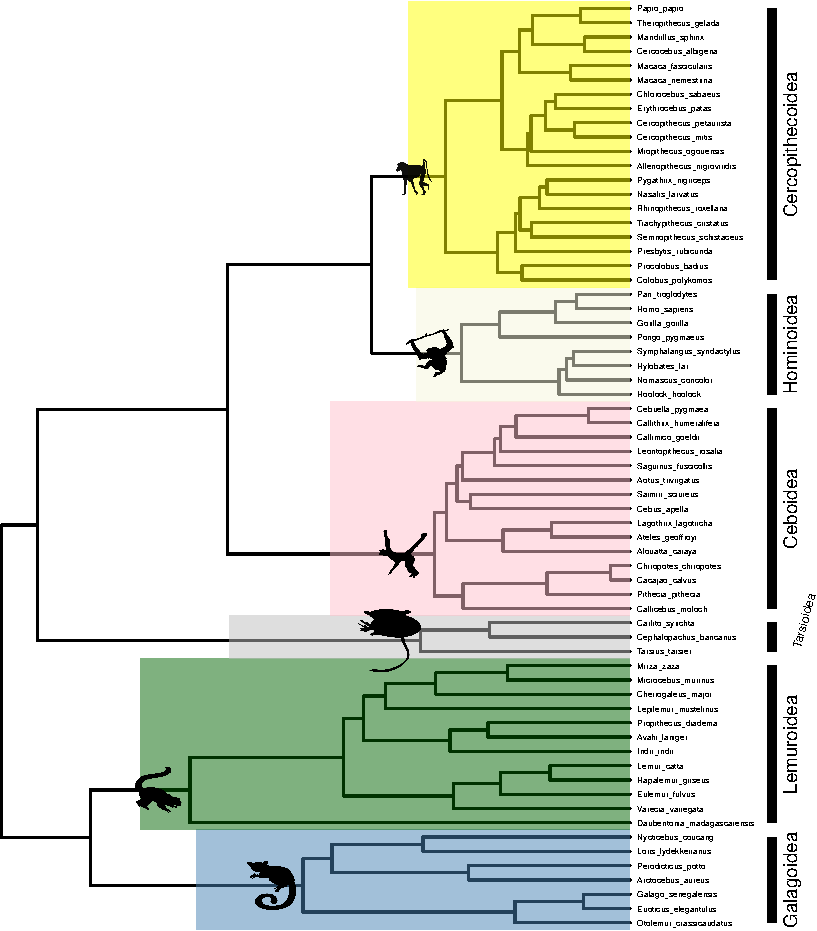
\includegraphics{bookdown-demo_files/figure-latex/unnamed-chunk-44-1.pdf}

As you can probably tell, the images don't have to be from Phylopic. You can use any images you have the rights to in exactly the same way!

\hypertarget{further-info}{%
\section{Further info}\label{further-info}}

This chapter barely scratches the surface of what ggtree is capable of. For much more detail, have a look at Guangchuang Yu's very own Bookdown covering the topic. You can access the book by clicking \href{https://yulab-smu.github.io/treedata-book/}{here} or by running the following code in R once you have ggtree installed.

\begin{Shaded}
\begin{Highlighting}[]
\KeywordTok{vignette}\NormalTok{(}\StringTok{"ggtree"}\NormalTok{, }\DataTypeTok{package =} \StringTok{"ggtree"}\NormalTok{)}
\end{Highlighting}
\end{Shaded}

\hypertarget{bibliography}{%
\chapter{Bibliography}\label{bibliography}}

  \bibliography{CRG.bib,book.bib,packages.bib}

\end{document}
